\documentclass{Phyport}

\usepackage{placeins}
\usepackage{hyperref}
\usepackage{amsmath}
\hypersetup{
    colorlinks=true,
}

\exname{万用表的设计} %实验名称
\extable{4}
\instructor{谭艾林} %指导教师
\class{github} %班级
\name{MJ} %姓名
\stuid{2025} %学号

\nyear{2025} %年
\nmonth{12} %月
\nday{22} %日
\nweekday{一} %星期几

\begin{document}
\setcounter{page}{0}
\makecover

\section{预习报告（10分）}
\subsection{实验综述（5分）}

万用表主要由直流电流计及若干电阻构成，本实验要设计指针式万用表，主要是由磁电式电流计以及一系列电阻组成。
其中电流计有两个主要参数，用 $I_g$ 表示电流计允许通过的最大电流， 用 $R_g$ 表示电流计线圈的电阻。

要改装量程为 $I$ 的电流表，需要在电流计两端并联一个分流电阻，阻值满足 $R_s = \frac{R_g I_g}{I-I_g}$ ，
选取不同的电阻即可构成不同量程的电流表。

当使用量程为 $I_g = 1 mA$ 的电流计改装为有 $5 mA$ 和 $10 mA$ 两个量程的电流表时，设计如图：
\begin{figure}[htpb!]
    \centering
    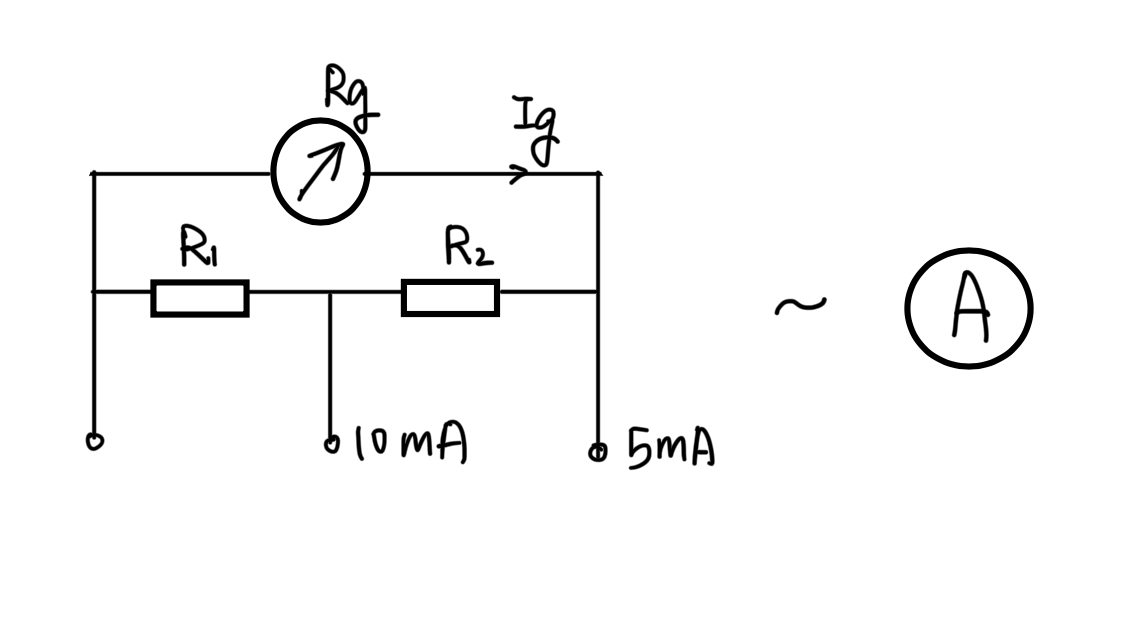
\includegraphics[width = 0.35\textwidth]{fig1.jpg}
\end{figure}

其中并联的电阻阻值满足：

\[
\begin{cases}
    (R_1 + R_2)(5 - I_g) = R_g I_g \\
    (R_2 + R_g) I_g = R_1 (10 - I_g)
\end{cases}
\]

然后使用标准安培表校正改装后的电流表，并分析误差，如图：
\begin{figure}[htpb!]
    \centering
    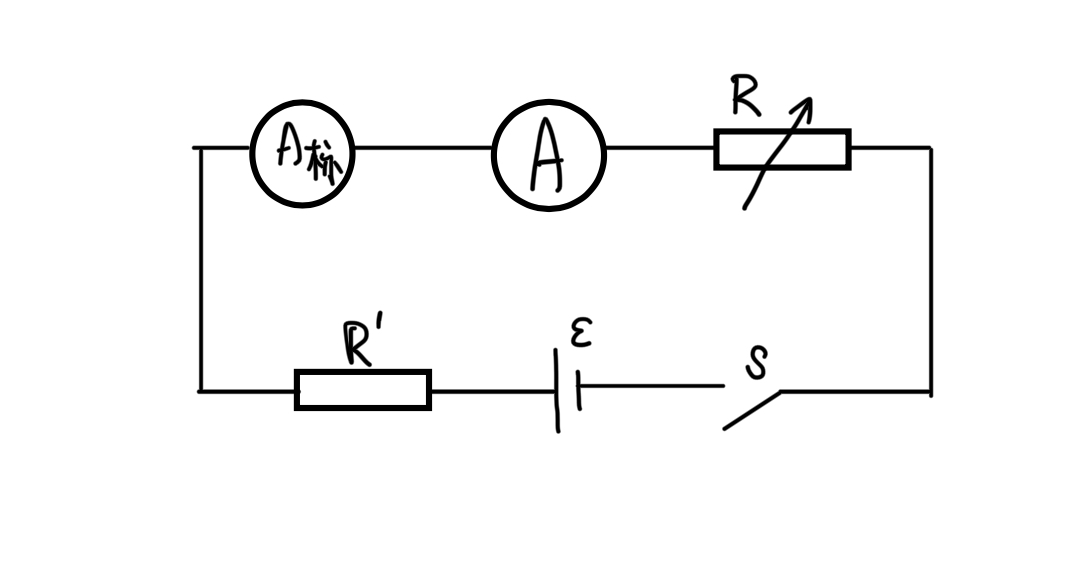
\includegraphics[width = 0.3\textwidth]{fig2.jpg}
\end{figure}

其中 $A_{\text{标}}$ 为标准安培表， $A$ 为改装电流表， $R$ 为可调节电阻， $R'$ 为限流保护电阻， $\epsilon$ 为直流电源。

要改装量程为 $U$ 的电压表，使用改装后的电流计并串联一个分压电阻，阻值满足 $R_x = \frac{U}{I_g'} - R_g'$ ，
其中 $R_g'$ 为电流计等效内阻， $I_g'$ 为电流计等效量程。

当要改装为有 $5V$ 和 $10V$ 两个量程的电压表时，设计如图：
\begin{figure}[htpb!]
    \centering
    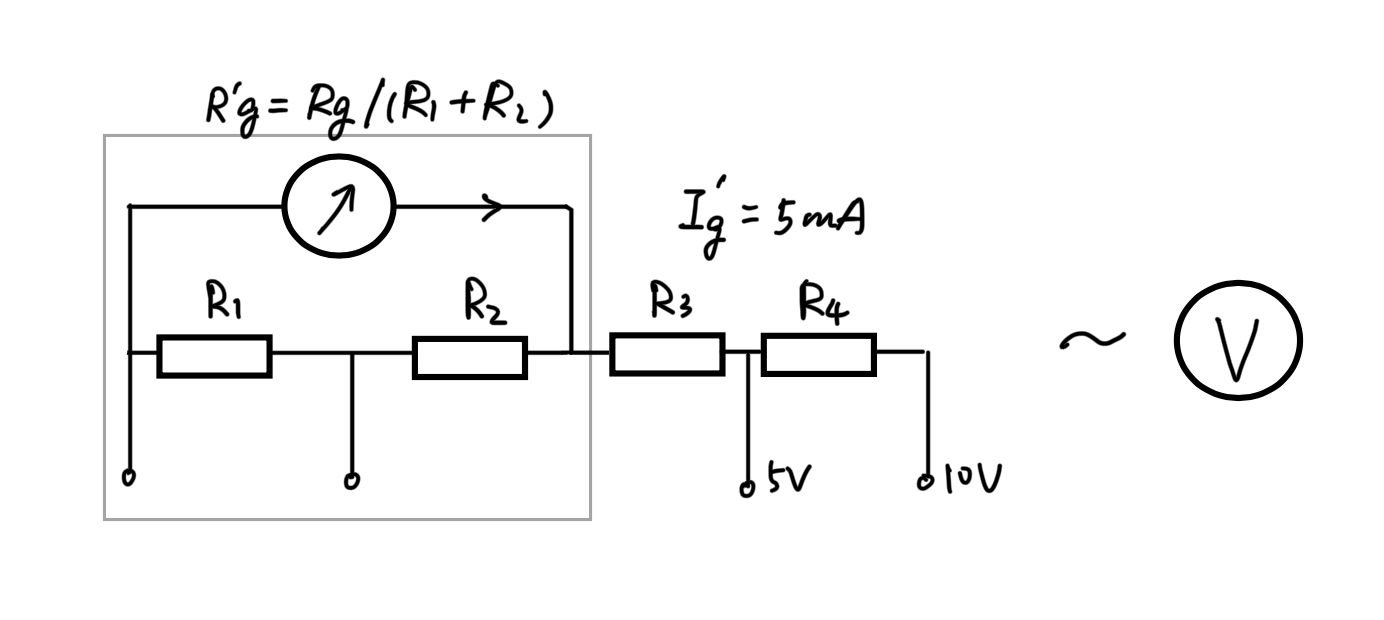
\includegraphics[width = 0.4\textwidth]{fig3.jpg}
\end{figure}

其中串联的电阻阻值满足：

\[
\begin{cases}
    I_g' (R_g' + R_3) = U_1 \\
    I_g' (R_g' + R_3 + R_4) = U_2     
\end{cases}
\]

然后使用标准伏特表校正改装后的电压表，并分析误差，如图：
\begin{figure}[htpb!]
    \centering
    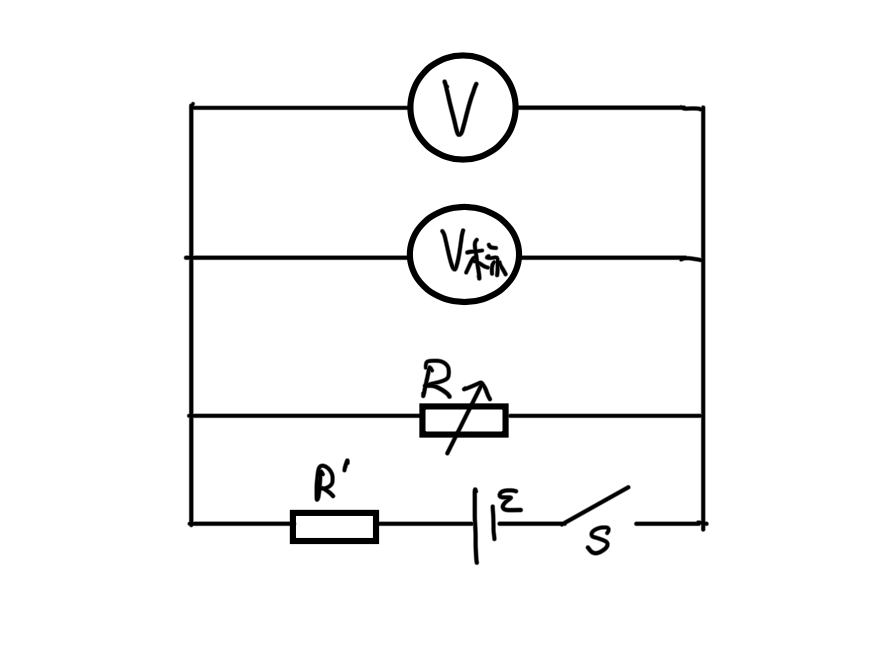
\includegraphics[width = 0.3\textwidth]{fig4.jpg}
\end{figure}

其中 $V_{\text{标}}$ 为标准伏特表， $v$ 为改装电压表， $R$ 为可调节电阻， $R'$ 为限流保护电阻， $\epsilon$ 为直流电源。


改装欧姆表时，需要短接 $a、b$ 两端并调节电阻 $R$ 使得电流计满刻度，此时满足 $\epsilon = I_0 (R_g' + R')$ ；
接入待测电阻后，回路满足 $\epsilon = I_x (R_g' + R' + R_x)$ 。当 $R_x = R_g + R'$ 时有 $I_x = \frac{I_0}{2}$ ，
此时电表指针指向刻度线中点，电阻 $R_x$ 称为欧姆表中值电阻，据此可以用电流计测量不同的电阻阻值。

此外由于电源电池非恒定，所以需要在电路中串联一电位器 $R_6$ 作零欧姆调整，如图：
\begin{figure}[htpb!]
    \centering
    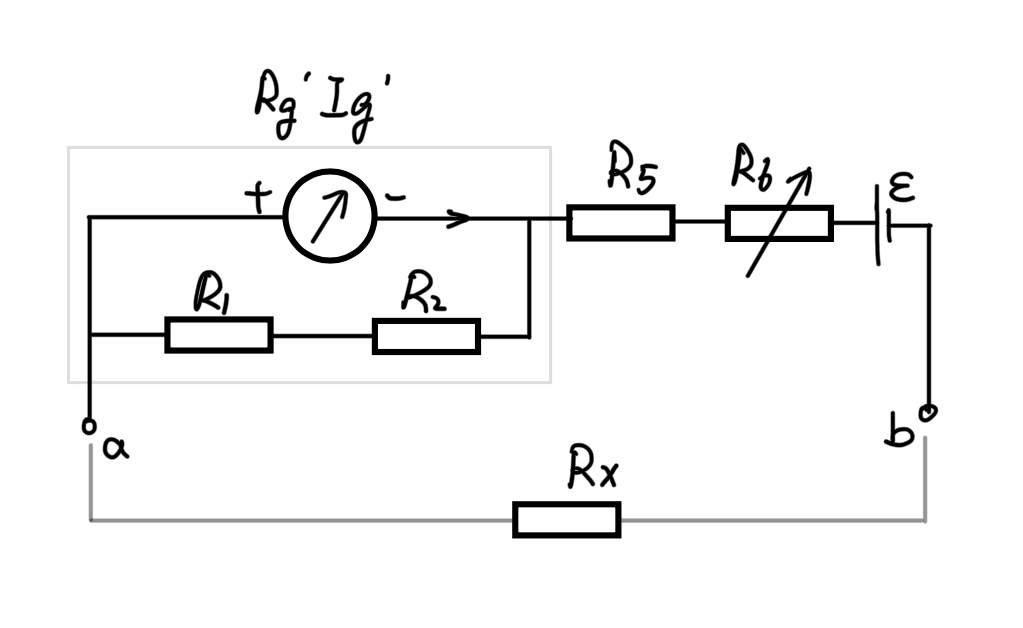
\includegraphics[width = 0.35\textwidth]{fig5.jpg}
\end{figure}

\subsection{实验重点（3分）}

本实验的重点在于了解指针式万用表的结构和测量电流、电压和电阻的基本原理，并掌握使用磁电式电流计改装多量程电流表、电压表和欧姆表的方法；
同时学习如何通过标准电表和可调节电阻校准万用表。

\subsection{实验难点（2分）}

本实验的难点在于准确计算和选取分流或分压电阻，因为有偏差会影响电表量程准确性；
改装后必须校准电表，控制电流或者电压稳定；在改装欧姆表时由于刻度非线性，设计要求较高；
此外需要考虑电流计内阻对电表的影响。

\section{原始数据（20分）}

实验记录数据：

\begin{figure}[htpb!]
    \centering
    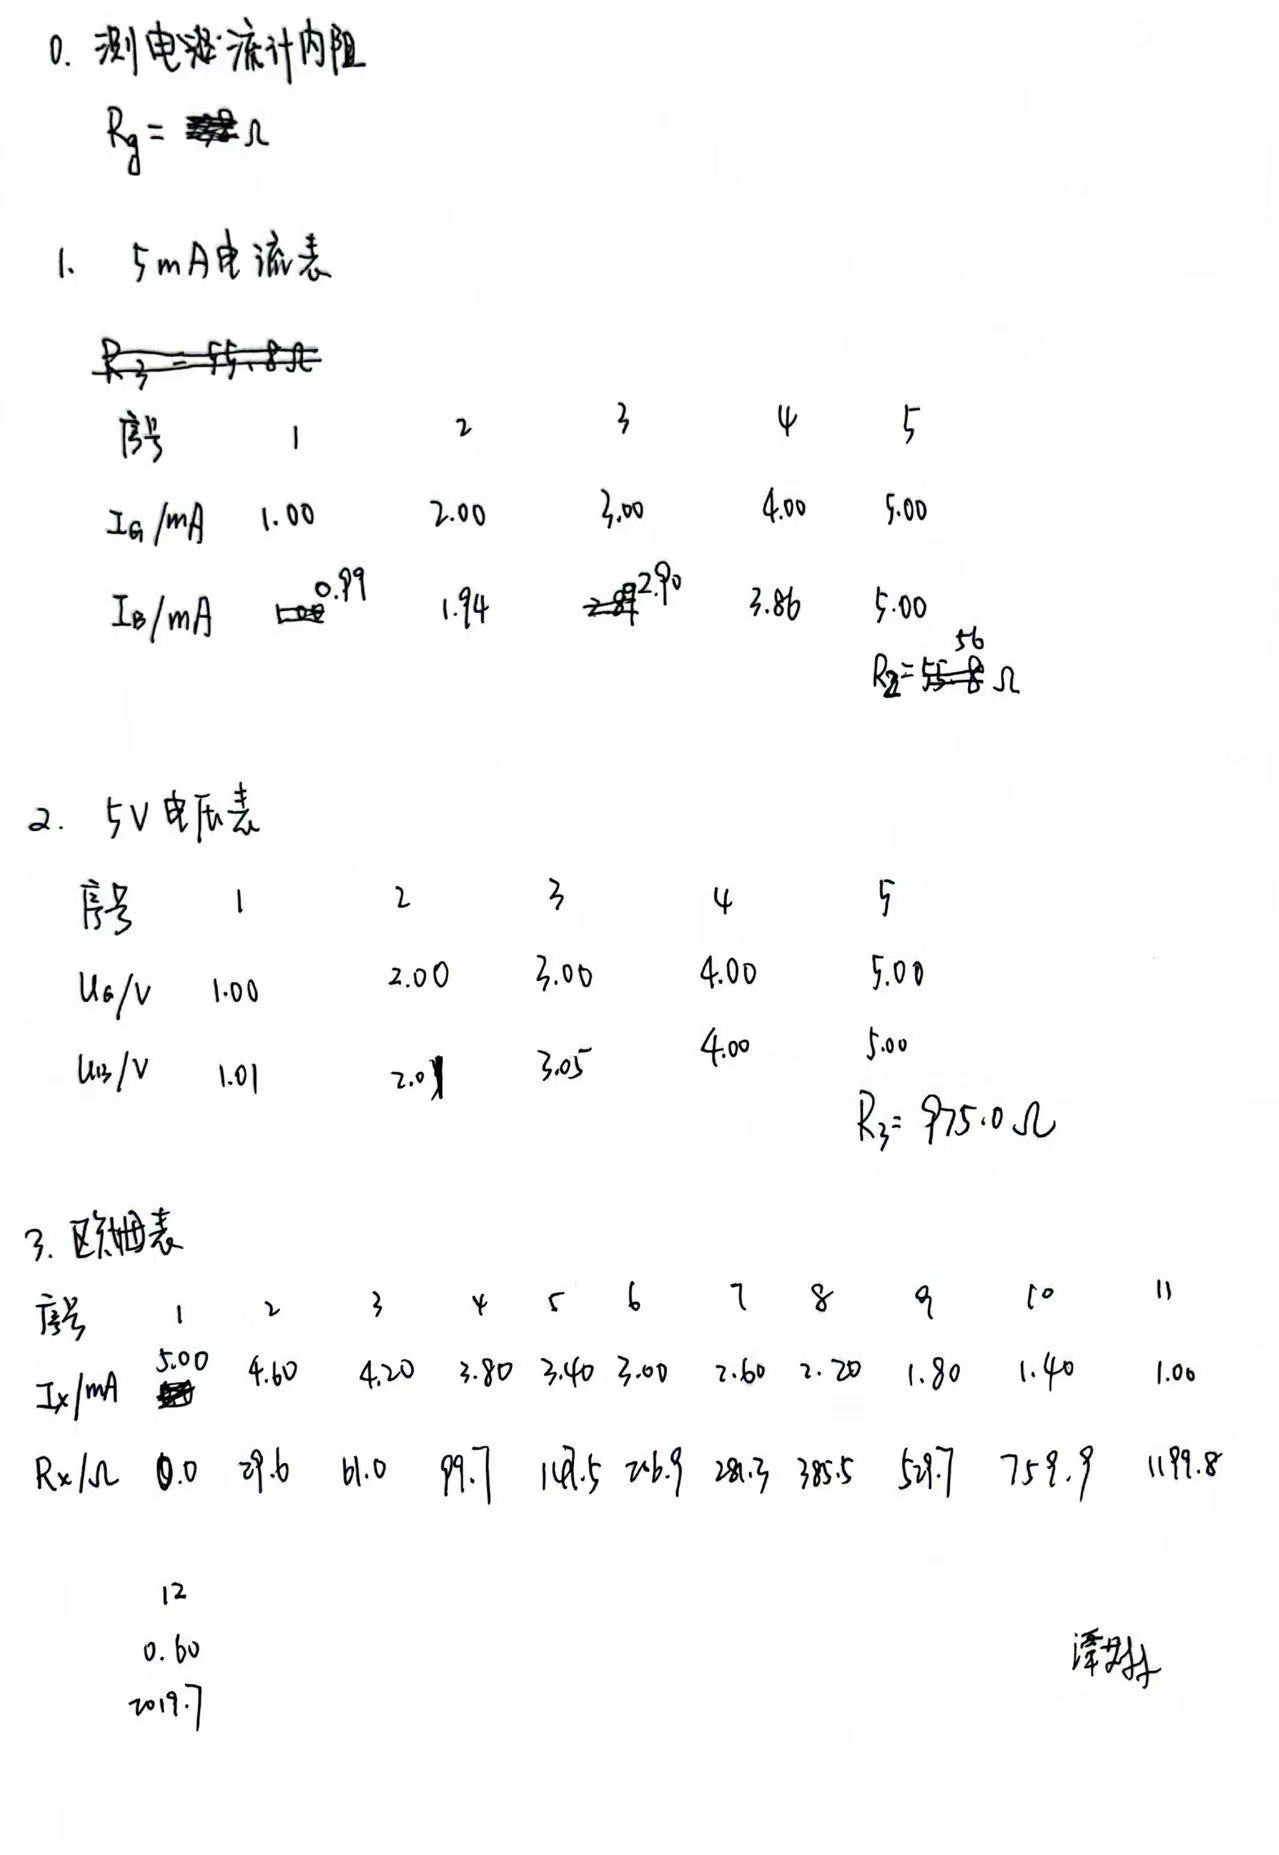
\includegraphics[width=0.85\textwidth]{data13.jpg}
\end{figure}

\section{结果与分析（60分）}
\subsection{数据处理与结果（30分）}

\textbf{1. 设计并改装 $5 mA$ 电流表}

对改装后的电流表进行校准，其中只使用一个并联电阻 $R_2 = 56 \Omega$ ，并且得到数据：

\begin{table}[htpb!]
    \centering
    \begin{tabular}{cccccc}
        \hline
        实验序号 & 1 & 2 & 3 & 4 & 5 \\
        \hline
        改装电流表读数 $I_g / mA$ & 1.00 & 2.00 & 3.00 & 4.00 & 5.00 \\
        标准安培表读数 $I_B / mA$ & 0.99 & 1.94 & 2.90 & 3.86 & 5.00 \\
        \hline
    \end{tabular}
\end{table}

使用MATLAB绘制 $I_g$ 和 $I_B$ 的关系曲线：

\begin{figure}[htpb!]
    \centering
    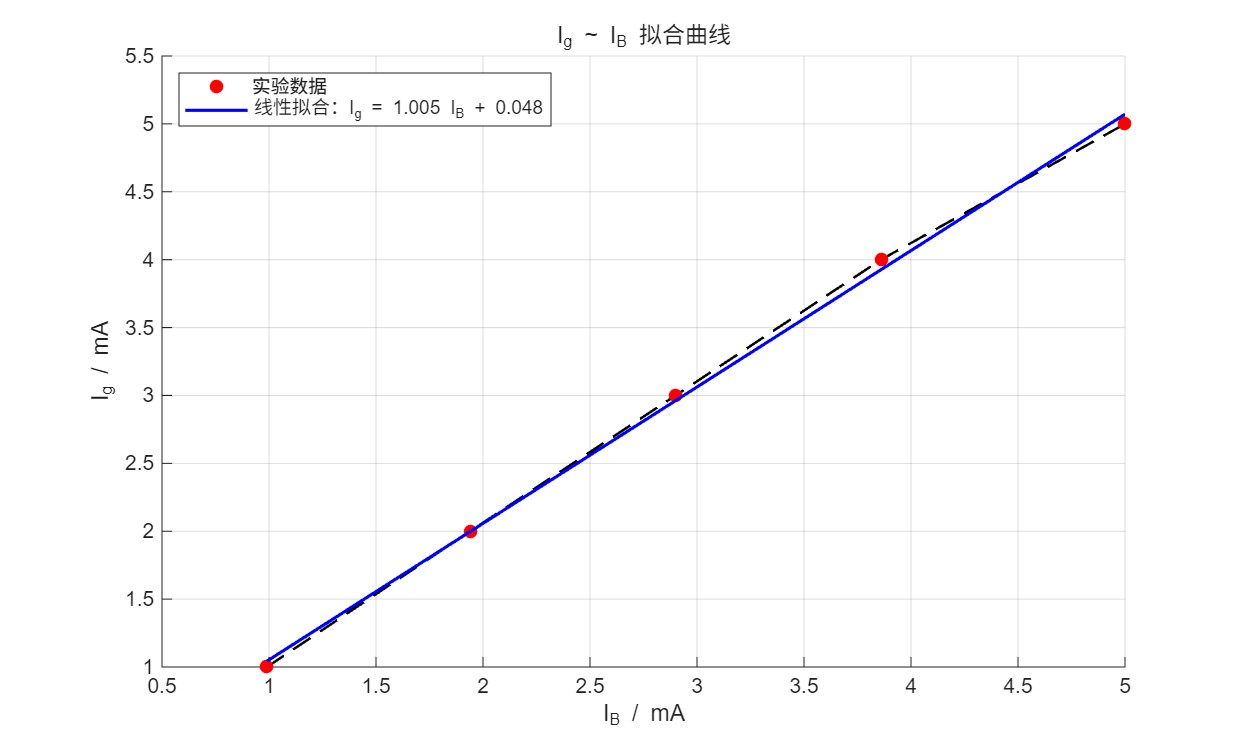
\includegraphics[width=0.6\textwidth]{fit13.jpg}
\end{figure}

计算改装电流表等级：

\[
K = \frac{\max {|I_g - I_B|}}{I_{\text{量程}}} \times 100 \% = 2.80 \%
\]

根据我国标准，这个改装电流表等级为 5.0 级。

\textbf{2. 设计并改装 $5 V$ 电压表}

对改装后的电压表进行校准，其中串联电阻 $R_3 = 975.0 \Omega$ ，并且得到数据：

\begin{table}[htpb!]
    \centering
    \begin{tabular}{cccccc}
        \hline
        实验序号 & 1 & 2 & 3 & 4 & 5 \\
        \hline
        改装电压表读数 $U_g / V$ & 1.00 & 2.00 & 3.00 & 4.00 & 5.00 \\
        标准伏特表读数 $U_B / V$ & 1.01 & 2.01 & 3.05 & 4.00 & 5.00 \\
        \hline
    \end{tabular}
\end{table}

使用MATLAB绘制 $U_g$ 和 $U_B$ 的关系曲线：

\begin{figure}[htpb!]
    \centering
    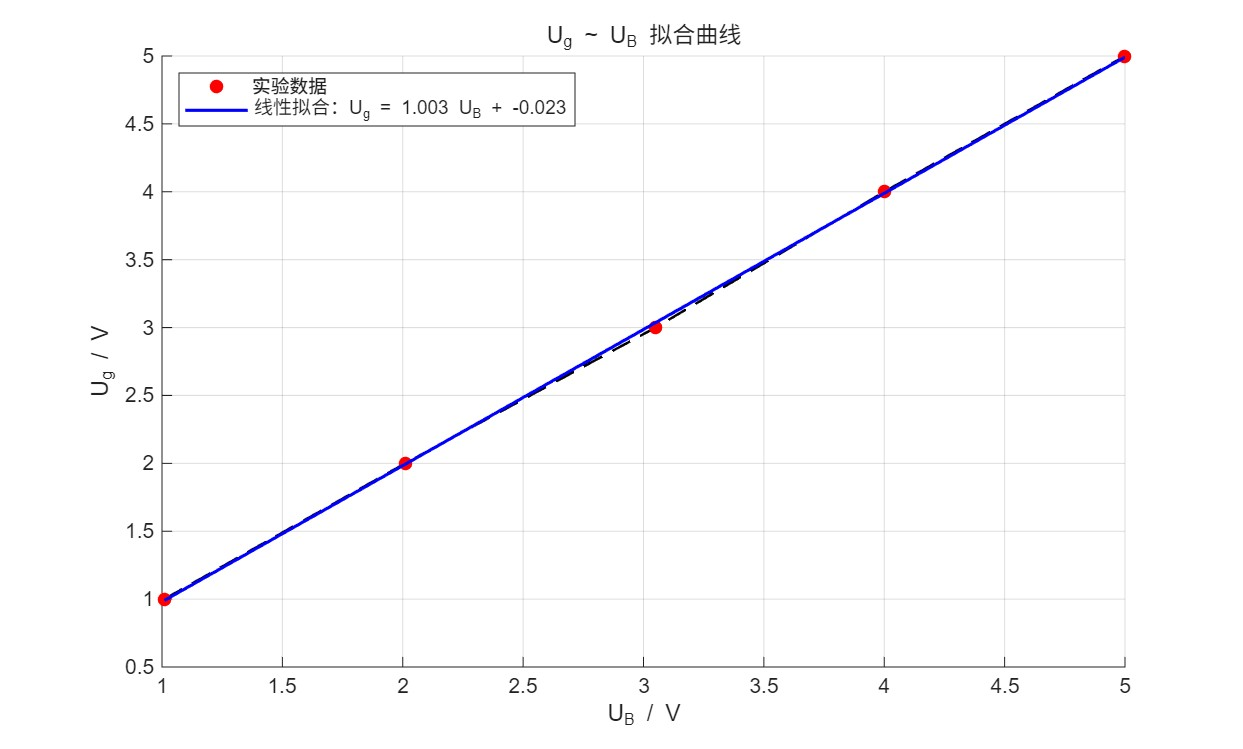
\includegraphics[width=0.6\textwidth]{fit13_2result.jpg}
\end{figure}

\FloatBarrier

计算改装电压表等级：

\[
K = \frac{\max {|U_g - U_B|}}{V_{\text{量程}}} \times 100 \% = 1.00 \%
\]

根据我国标准，这个改装电压表等级为 1.0 级。

\textbf{3. 设计并改装欧姆表}

将可调电阻接入改装好的欧姆表，得到测量数据：

\begin{table}[htpb!]
    \centering
    \begin{tabular}{ccccccc}
        \hline
        实验序号 & 1 & 2 & 3 & 4 & 5 & 6 \\
        $I_x / mA$ & 5.00 & 4.60 & 4.20 & 3.80 & 3.40 & 3.00 \\
        $R_x / \Omega$ & 0.0 & 29.6 & 61.0 & 99.7 & 147.5 & 206.9 \\
        \hline
        实验序号 & 7 & 8 & 9 & 10 & 11 & 12 \\
        $I_x / mA$ & 2.60 & 2.20 & 1.80 & 1.40 & 1.00 & 0.60 \\
        $R_x / \Omega$ & 281.3 & 385.5 & 529.7 & 759.9 & 1199.8 & 2019.7 \\
        \hline        
    \end{tabular}
\end{table}

使用MATLAB绘制 $I_x$ 和 $R_x$ 的关系曲线：

\begin{figure}[htpb!]
    \centering
    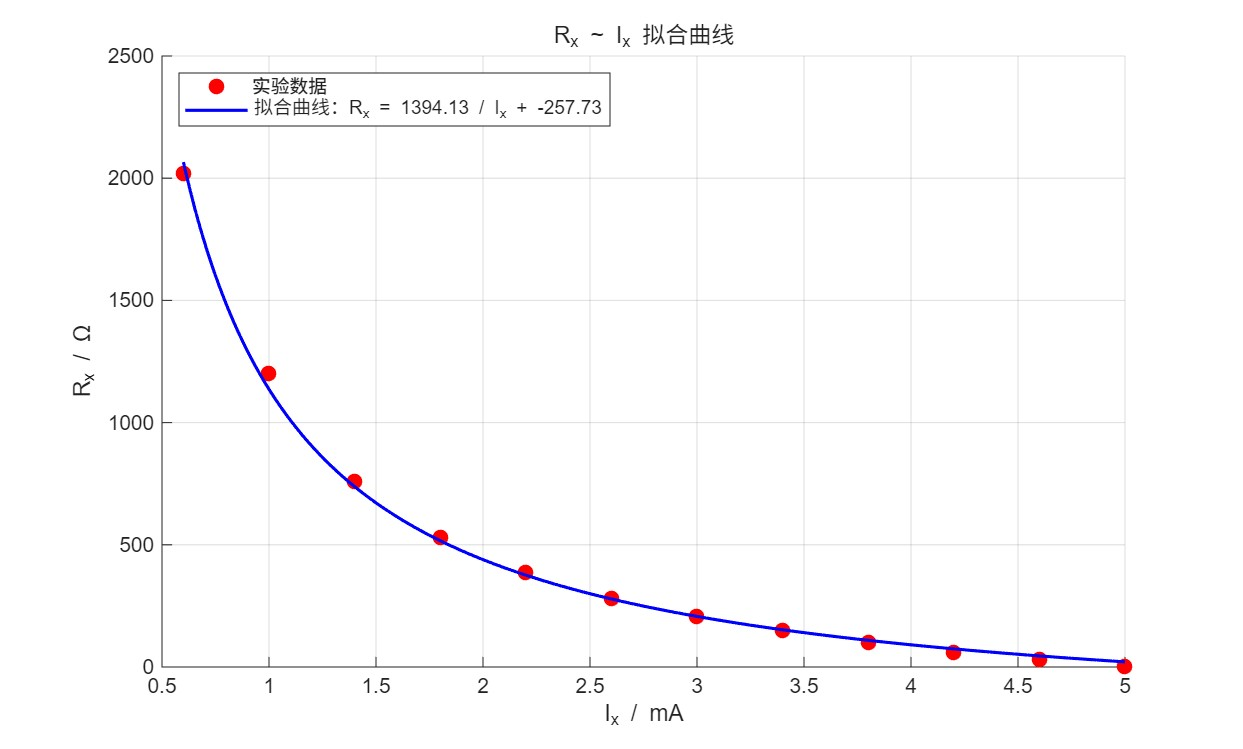
\includegraphics[width=0.6\textwidth]{fit13result3.jpg}
\end{figure}

结合测量数据和图像来看，改装欧姆表的刻度呈现非线性分布，相同电流变化对应的电阻变化不相等。在低电阻区间，电阻变化较小即可引起电流的明显变化，因此刻度分布较为密集；
而在高电阻区间，电流变化趋于平缓，相同的电流变化对应较大的电阻变化，刻度逐渐变得稀疏。此外，
改装欧姆表在中等电阻范围内具有较高的测量灵敏度。


\subsection{误差分析（20分）}

根据改装万用表等级和测量结果来看，这个实验的误差主要来源于：

1. 接入的导线存在电阻，对电流和电压的测量产生一定影响；

2. 校准电表时，标准电表和改装电表的指针都不是十分稳定，以及无法完全同时达到满偏位置，因此影响改装电表的精确性；

3. 读数时存在视差，或者存在一定主观性，影响测量结果；

4. 改装万用表时使用的可调电阻不是连续变化的，同时电流计和标准电表的精度不够高，有一定误差。

\subsection{实验探讨（10分）}

本实验依据指针式万用表测量电流、电压和电阻的基本原理，主要使用电流计对电流表、电压表及欧姆表进行改装与标定。
实验中根据电学相关知识进行电路设计、电阻选取与电路连接。实验结果表明，改装电流表和电压表具有较好的线性关系，
而欧姆表由于其工作原理呈现明显的非线性刻度特征。

\section{思考题（10分）}

\textbf{1. 为什么不能用万用表欧姆档测量电源内阻？}

因为万用表欧姆档通过内部电源提供固定电压测量电阻，本质上是根据测得的电流大小来确定阻值，
而被测电源本身存在电动势，万用表电压会干扰电源工作状态，导致测量电流与实际负载电流不符，从而产生错误读数。

\textbf{2. 为什么不能用欧姆表测量另一表头内阻？}

因为欧姆表的电阻刻度不均匀，测量电阻需要估读，精确度较低；而用表头改装电表时，对阻值的测量精度要求较高，
不应该用欧姆表直接测量其内阻，而且考虑到表头量程很小，测量时可能会超过量程，不安全。

\textbf{3. 为什么 $I_x$ 与 $R_x$ 为非线性关系？}

因为欧姆表通过内部电源提供电压，根据电流大小判定电阻，满足：

\[
I_x = \frac{\epsilon}{R_0 + R_x}
\]

即指针电流和被测电阻呈反比例关系，随着 $R_x$ 增大，分母增大导致电流变化幅度减小，从而形成低阻区刻度密集、高阻区刻度稀疏的非均匀刻度特征。

\begin{thebibliography}{9}
    \bibitem{ref1}
    全国电工仪器仪表标准化技术委员会(SAC/TC 104). 直接作用模拟指示电测量仪表及其附件  第1部分:定义和通用要求:GB/T 7676.1-2017[S]. 质检出版社. 2017. 

\end{thebibliography}

\input{注意事项}
\end{document}
